\documentclass[article]{article}
\usepackage{amsmath,amsthm,bm,mathrsfs,amssymb}
\usepackage[a4paper, total={6in, 9in}]{geometry}
\usepackage{graphicx, subcaption}
\usepackage[colorlinks]{hyperref}
\usepackage{multirow,tabularx}
\newcolumntype{Y}{>{\centering\arraybackslash}X}
\title{Numerical Algorithms – Assignment 2}
\author{Kahaan Shah \& Santripta Sharma}
\date{\today}

\setlength{\parindent}{0pt}

\begin{document}

\maketitle

\section{Introduction}
For this assignment we have implemented Latent Semantic Indexing on a dataset of books from the Ashoka library. The goal of the assignment is to index book categories according to the \href{https://en.wikipedia.org/wiki/Dewey_Decimal_Classification}{Dewey Decimal System} which categorizes books by their discipline into 9 broad categories (0-9), followed by subcategories in each increasing unit place in the code. For example a Dewey Decimal Number (DDN) of 331 indicates that a book is under 300 (social sciences), 330 (economics) and 331 (labour economics). Books are assigned a number depending on how broadly or narrowly they can be categorised. 

\section{Data}
We used a data set of about 10000 books pulled from the \href{https://koha.ashoka.edu.in}{Ashoka Library Catalogue}. Books were pulled with their title as well as their DDN.

\section{Latent Semantic Indexing}

\subsection{Term-Document Frequency Matrix}

We constructed three different matrices as specified below. In each matrix the columns represented document vectors, and rows represented term vectors. For our implementation we considered the Dewey Decimal Categories as the documents, essentially concatenating all titles in a given category. So $\mathbf{A}_{ij}$ is the relationship of term $i$ with document $j$ as defined differently for each matrix below:

\begin{enumerate}
    \item Frequency matrix: $\textbf{A}_{ij}$ is the frequency of term $i$ in book titles for the category $j$. 
    \item Normalised frequency matrix: $\textbf{A}_{ij}$ is the frequency of term $i$ in book titles for the category $j$ divided by the total occurrences of the term across all titles. 
    \item Binary frequency matrix: $\textbf{A}_{ij}$ is 1 if term $i$ occurs in category $j$, 0 otherwise.
\end{enumerate}

We used termdoc matrices of size $10103 \times 521$, i.e., we had a dictionary of size $10103$ and $521$ Dewey Decimal Categories. Next, we use SVD to perform latent topic discovery.

\subsection{Latent Topic Discovery using Truncated SVD}
The idea here is to construct a low rank approximation to $\bf A, A_k$ of rank $k$. We can arrive at this by performing an SVD on $\bf A$, and truncating this to the largest $k$ singular values and their associated singular vectors.\bigskip

We decomposed each of the matrices using thin-SVD which yielded $\mathbf{U} \in \mathrm{R}^{10103 \times 521}$, $\mathbf{\Sigma} \in \mathrm{R}^{521 \times 521}$, $\mathbf{V}^t \in \mathrm{R}^{521 \times 521}$.

\subsubsection{Latent Space Visualisation}{
To visualise the indexed vectors we plotted the term representations from $\mathbf{U}$ in the first two latent dimensions, i.e. plotting each column in $\mathbf{U}$ in the first two dimensions, scaled by their respective singular values. The plots for these are shown below.

\begin{figure}[h]
    \centering
    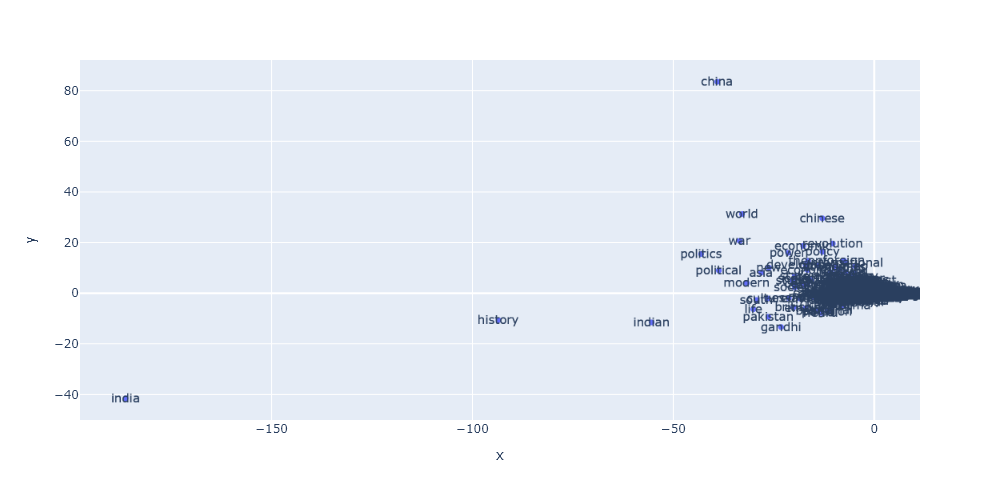
\includegraphics[width=0.9\linewidth]{freq_term_space.png}
    \caption{Frequency Term Space}
    \label{fig:freqterms}
\end{figure}

\begin{figure}[h]
    \centering
    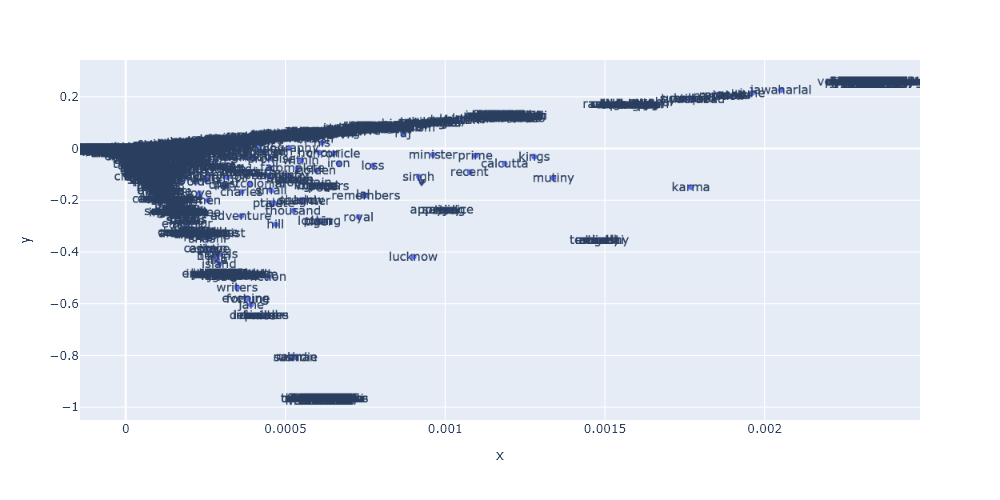
\includegraphics[width=0.9\linewidth]{norm_term_space.png}
    \caption{Normalised Term Space}
    \label{fig:normterms}
\end{figure}

\begin{figure}[h]
    \centering
    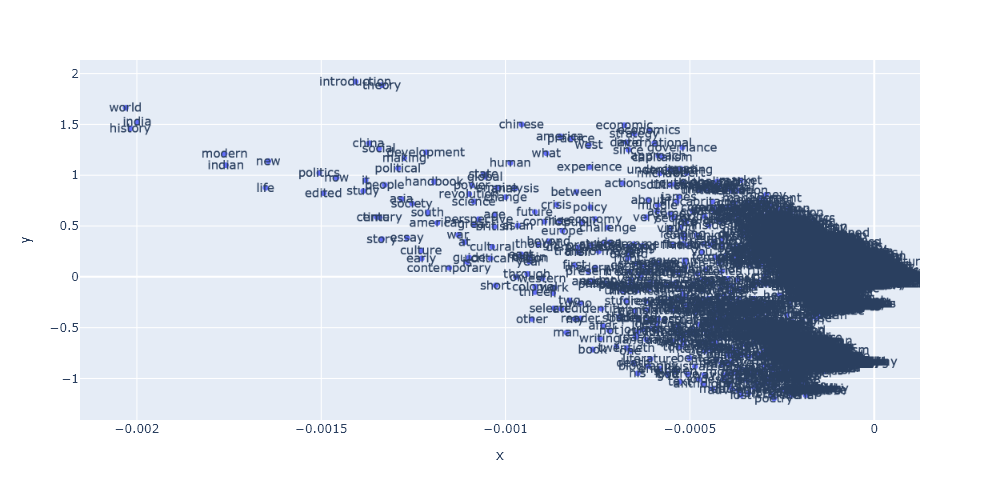
\includegraphics[width=0.9\linewidth]{bin_term_space.png}
    \caption{Binary Term Space}
    \label{fig:binterms}
\end{figure}
}

While the different methods of weighing the term doc elements seems to give wildly disparate term spaces, there is a similarity between the binary and frequency based approaches, in terms of recognising similar term correspondences. For instance, they both show terms related to "India" as outliers on the first principal component (plotted as x) here, and (somewhat) cluster them, in terms of nearest neighbours, with terms like "politics", "world", "history", "modern", etcetera, which is the expected result, due to the high frequency of their co-occurrence.\bigskip

Similarly, in both the frequency \& binary approaches, "economy", "theory", "development", "policy", and "power" are clustered together.\bigskip

In the normalised approach, it is difficult to detect any salient clusters, due to the much tighter spread of the terms on the second principal component (y-axis here).\bigskip

Another point to recognise is that this 2D representation of our space misses out a lot of detail (all the separation on the other principal components), and therefore doesn't allow us to definitively claim much about the comparative quality of the three approaches, unless we plan to truncate the SVD to $2$ terms.

\subsubsection{Rank Analysis} {
First, we look at the ratios of the largest and smallest singular values for each matrix:

\begin{center}
    \begin{tabular}{|c|c|c|c|}
        \hline \textbf{Matrix} & $\sigma_1$ & $\sigma_{521}$ & $\sigma_1\div\sigma_{521}$ \\
        \hline Frequency & 277.765 & 1.223e-15 & 2.265e+17 \\
        \hline Normalised & 20.281 & 9.007e-15 & 2.252e+15 \\
        \hline Binary & 60.885 & 2.468e-16 & 2.466e+17 \\
        \hline
    \end{tabular}    
\end{center}

Given the large relative distance between the largest and smallest singular values in each case, the termdoc matrix should admit a "stable" low-rank approximation. However, we also notice that this large relative difference only occurs with the last term. If we instead consider the ratios of consecutive singular values, $\sigma_n / \sigma_{n+1}$, we only see this ratio be larger than $10$ for the last ratio (i.e. $\sigma_{520}/\sigma_{521}$) for all matrices, giving us no clear truncation point.\bigskip

Nonetheless, latent semantic indexing relies on a dimensionality reduction to reveal the latent topic space, so we choose a set of ranks, $k \in \{ 8, 16, 32, 65, 130, 260, 520, 521 \}$, to truncate our decompositions to, so we may compare results between different truncation factors.
}

\subsection{Queries}

The goal of querying this index would be to provide a set of terms and identify which category one must look in to find books of that term. Alternatively, given an unclassified book's title as the query, it provides an estimate for which category that book would best fit in with. Since a query of terms is essentially the same as a document we encode query vectors in the same manner as document (category) vectors. To project so, for a query vector $\mathbf{q}$, we have the representation $\hat{\mathbf{q}} = \mathbf{q}^t \mathbf{U} \mathbf{\Sigma}^{-1}$. We are essentially finding the relationship between the query vector and each of the term vectors, then scaling each component by the multiplicative inverse of the associated singular value.

\section{Results and Observations}

Here, we display the results of various queries against different values of $k$ (the truncated rank) and the weighting approach used. Note that we have converted the numbers from the DDN categories to their labels for easier interpretation:\bigskip

\begin{tabularx}{\textwidth}{|*{7}{Y|}}
\hline
\multirow{2}{*}{Query} & \multicolumn{2}{c|}{Freq} & \multicolumn{2}{c|}{Norm} & \multicolumn{2}{c|}{Bin}\\
\cline{2-7} & $32$ & $130$ & $32$ & $130$ & $32$ & $130$\\
\hline 
Linear Algebra & Algebra \& Number Theory & Algebra \& Number Theory & Algebra \& Number Theory & Algebra \& Number Theory & Analysis & Algebra \& Number Theory\\
\hline
Ambedkar & Social groups & Civil \& political rights & Social groups & Civil \& political rights & Social processes & Civil \& political rights\\
\hline
Textile Industry & Intl. commerce & Public finance & Production & Textile arts & Production & Intl. commerce\\
\hline
Machine Learning & Military science &  Schools \& their activities & Military science & Military science & Military science & Military science\\
\hline
Social Media & Social processes & Social interaction & Social interaction & Social interaction & Social interaction & News media, journalism \& publishing\\
\hline
First Past the Post & English fiction & Mental processes \& intelligence & Political science & Mental processes \& intelligence & Political science & Mental processes \& intelligence\\
\hline
\end{tabularx}\bigskip

Our first observation was that there seems to be a convergence towards the same label across all approaches as $k \rightarrow 521$ (though it is hard to display here), but they converge at different speeds. A smaller version of this can be seen here as well, for example, in the second and last queries.

There are, of course, some queries where we observe the opposite effect of divergence, eg. the third query.\bigskip

We should also note that if instead of taking only the first document returned for these queries, we take the set of the first 5, there is a large overlap between all methods and between values of $k$. This is, once again, hard to display in a tabular format, and thus excluded here.

\subsection{Validation: Mislabelling Error}
Here, we devise an experiment to gauge the accuracy of our retrieval "models". We ask each model to classify every title we have into a DDN category. We give it an error, based on the most significant digit that deviates from the actual/ground truth category. To illustrate this, assume our ground truth label is $312$. Then, the prediction $512$ has an error of $3$, $300$ has an error of $2$, $315$ has an error of $1$ and $312$ has an error of $0$.\bigskip

We average this error over all titles we know of, and report that below. \textbf{Note that this is not using a train/test split}, since the "models" are "trained" on each title, and therefore we expect to see some "overfitting". However, if the truncated representations are able to achieve similar (or better) mean errors, we say they successfully capture a low-dimensional representation of the space. We report our metrics below:\bigskip

\begin{center}
    \begin{tabular}{|*{4}{c|}}
    \hline $k$ & Frequency & Normalised & Binary\\
    \hline $8$ & 1.834 & 1.936 & 1.922\\
    \hline $16$ & 1.576 & 1.729 & 1.734\\
    \hline $32$ & 1.468 & 1.536 & 1.448\\
    \hline $65$ & 1.305 & 1.278 & 1.167\\
    \hline $130$ & 1.333 & 1.092 & 1.110\\
    \hline $260$ & 1.553 & 1.068 & 1.286\\
    \hline $520$ & 1.960 & 1.548 & 1.652\\
    \hline $521$ & 2.519 & 1.902 & 2.116\\
    \hline
    \end{tabular}
\end{center}

Out main observation here is that the trend across all three is that there is a certain optimal value for $k$ above and below which the LSI performs worse. We also see that the normalised matrix reaches the lowest error as we increase $k$ after a certain dimension. Overall, the error is mostly below 2, indicating that the LSI is atleast able to identify the broad categories of books, and in the best case is able to categorise accurately into subcategories as well. Note that currently we are only evaluating against the top prediction, but we expect the correct category to be predicted in the top 5 predictions.

\end{document}